\documentclass{article}

\usepackage{amsmath}
\usepackage{fancyhdr}
\usepackage{graphicx}
\graphicspath{{}}

%% some colours
\usepackage{color}
\definecolor{deepblue}{rgb}{0,0,0.5}
\definecolor{deepred}{rgb}{0.6,0,0}
\definecolor{deepgreen}{rgb}{0,0.5,0}
\definecolor{backcolour}{rgb}{0.95,0.96,0.93}

%%%%%%%%%%%%%% CODE STUFF %%%%%%%%%%%%%%
%%%%%%%%%%%%%%%%%%%%%%%%%%%%%%%%%%%%%%%%
\usepackage{cprotect} % to be used in sol
\usepackage{listings} % for code display
% setting code style
\newcommand\pythonstyle{\lstset{
        language=Python,
        backgroundcolor=\color{backcolour},
		basicstyle=\footnotesize,
		otherkeywords={self},
		keywordstyle=\footnotesize\color{deepblue},
		emph={__init__},
		emphstyle=\footnotesize\color{deepred},
		stringstyle=\color{deepgreen},
		frame=single,
		showstringspaces=false  ,
		breaklines=true,
		numbers=left,
		numberstyle=\footnotesize,
		tabsize=4,
		breakatwhitespace=false
	}}

% Python environment
\lstnewenvironment{python}[1][]{
    \pythonstyle
    \lstset{#1}
}{}

% Python for external files
\newcommand\pythonexternal[2][]{{
    \pythonstyle
    \lstinputlisting[#1]{#2}
}}

% Python for inline
\newcommand\pythoninline[1]{{\pythonstyle\lstinline!#1!}}

%%%%%%%%%%%%%%%%%%%%%%%%%%%%%%%%%%%%%%%%
% setting the style for ex documents
\pagestyle{fancy}
\fancyhf{}
\fancyhead[L]{\thetitle}
\fancyhead[C]{}
\fancyhead[R]{\theauthor}
\renewcommand{\headrulewidth}{0.4pt} %obere Trennlinie
\fancyfoot[L]{Due: \thedate}
\fancyfoot[R]{\thepage} %Seitennummer
\renewcommand{\footrulewidth}{0.4pt}

% include solutions
\newcommand\sol[1]{{\large\textbf{\\Solution:}}#1}
\usepackage{setspace}
\usepackage{enumerate}

\title{BPP Exercise 12 - Python and Experiments}
\author{A. Hain, M. Nipshagen}
\date{26.06.2018, 14:00}


\makeatletter
\let\thetitle\@title
\let\theauthor\@author
\let\thedate\@date
\makeatother


\newcommand\itemsub[1]{
	\begin{itemize}
		\item #1
	\end{itemize}
}

% do not include solutions
\renewcommand\sol[1]{}


\begin{document}

The deadline for this exercise sheet is \textbf{Monday, \thedate.}

\section*{Introductory Words}
Remember that you need proper documentation to pass
the homework. The documentation doesn't need to be \textit{perfect}, but
everything that needs a docstring, should have a docstring.\\
Make sure that your code does not crash on execution! If your code is not
runnable -- and especially if it is only a typo, and there are no comments
to explain your idea or why it was not fixable \textbf{we will consider that
particular task as failed}.\\
Task 1 and 2 are not dependent on each other. We supplied data to do task 2.

\section*{Precautions}
Install one of the frameworks -- either PsychoPy or Expyriment.\\
% It might be advantageous to setup a new conda environment (if you are using
% conda at all), so you do not mess with your working installation.
% To set up a new conda environment named \texttt{psy} type the following
% into your terminal: \verb|conda create -n psy|\\
% Then type \verb|activate psy| or if you are on UNIX \verb|source activate psy|.
% Now the psy environment is active, but you need to reinstall your libraries.
% So next type \verb|pip install numpy matplotlib pandas|.
You can install them via pip easily by using either
\verb|pip install expyriment| or
\verb|pip install psychopy|. In the best case this will run without errors, and
the library should be installed and you can proceed with setting up your experiment!


\section{The Great Experiment}
Let's design a small experiment: We want to find out whether we take longer
to react to a stimulus the farther it is away from the center of our vision.\\
The experiment will go as follows: we are constantly showing a fixation stimulus
in the middle of the screen and then display a circle after a (seemingly) random
amount of time between 1 and 6 seconds at a (seemingly) random position.
The subject will keep their eyes fixated on the stimulus in the middle and press
the left or the right key whenever they notice a circle appearing.
After the key press, the offset of the stimulus from the middle of the screen
and the reaction time (in milliseconds) will be logged to a .csv file.\\

\subsection{Guidelines and technical stuff}
\begin{itemize}
	\item Make the experiment be displayed in a \texttt{1024x768} WINDOW with a 
		light grey background.
	\item The fixation stimulus is a black small circle or cross in the center of the window.
	\item You can choose the exact size of the circles, but the radius should
		be around 25px. The circles will be completely black, meaning black outline and fill.
	\item There will be \textbf{one block} with \textbf{10 trials} (for simplicity). You predefine
		the single trials -- each subject has to see the exact same
		combinations of circle positions and offset times (the times after which the
		circles are shown), but for each subject you randomize order in which these
		position-timing tuples will appear.
	\item The experiment will exit after the user pressed the 'q' key (for 'quit')
	\item We came up with some conditions for you so you don't have to. The time
	values for the pause are in seconds, and the circle position is in pixels, 
	Set the units in your code and configurations accordingly where appropriate.
		\begin{tabular}{c|cc}
			time offset (pause) & circle position x & circle position y \\
			\hline
			4.5 & 128 & 64\\
			2.5 & 200 & 200\\
			5 & -256 & -192\\
			1 & 256 & -350\\
			5 & -200 & 200\\
			2.25 & -128 & 350\\
			2.5 & 200 & -200\\
			1 & -128 & -64\\
			4 & -450 & 0\\
			2 & 450 & 0

			
		\end{tabular}
	\item Most importantly: You can choose whether you want to use PsychoPy or 
		Expyriment to implement this program! Depending on which you choose, pay 
		attention to the programming and structure guidelines we've formulated for
		the respective library.
\end{itemize}

\subsection{Onto the Coding}
\noindent Now that everything important has been said, you would already be free to
program your experiment. With the following subtasks we are providing a
guideline of how you could tackle this task. You don't have to follow these,
but we strongly recommend it. You can also use these as checkpoints for your task.

\begin{enumerate}[a)]
\item The Window\\
No experiment without a window.
First, define your experiment window (and other necessities you might need to
principally run the experiment). Take a look at the guidelines for what the window
should look like and implement it accordingly.\\
Run your experiment to make sure it works (at this point, not much will happen --
this is to make sure your code is not crashing).

\item Stimuli Part 1\\
Now define the fixation stimulus. Draw it in the middle of the screen.
Make the program wait for a key input from the user after drawing, so you can
check if it worked. So the experiment should open, you should see a window with
the fixation stimulus in the middle and upon pressing some key, the program
should close again.\\
Run your code to see if the experiment behaves correctly.

\item Stimuli Part 2\\
Now define the circle stimulus. For now, draw it somewhere on the screen, but
at a different position from the cross, so they don't overlap each other.
Run your code and make sure the fixation and the circle can be shown at the 
same time.

\begin{figure}[h!]
	\centering
	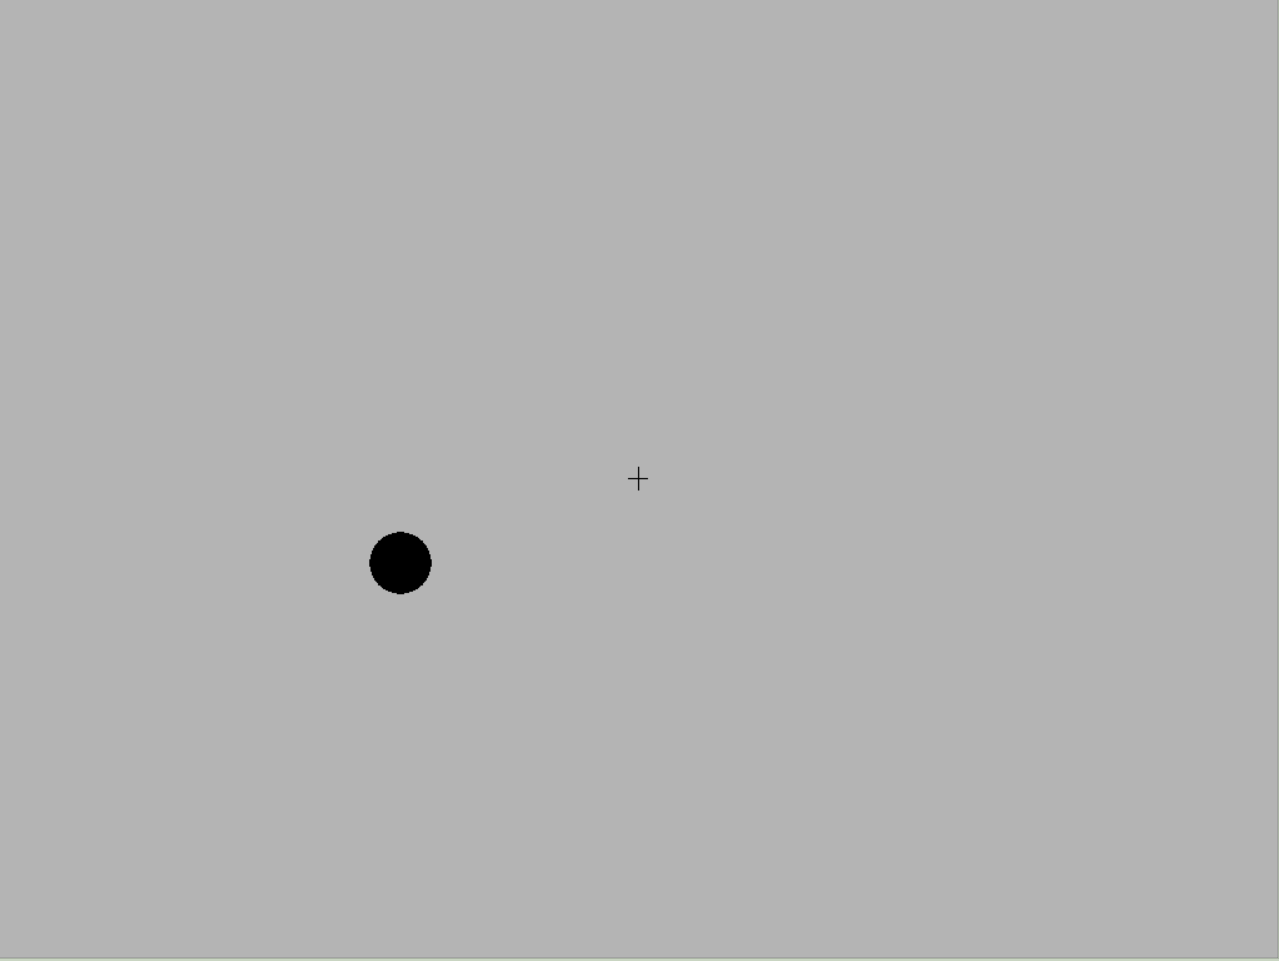
\includegraphics[width=.6\textwidth]{screen1}
	\caption{An example how it could look after Stimuli Part 2}
\end{figure}

\item The Loop\\
Include the circle position and time offset conditions into your code. You might
want to use a dictionary and a list for this. In the list, store the keys
of the dictionary. This is what you will iterate over in your experiment.
You can simply use the integer from 1 to 10 (the trial numbers) as keys.
The corresponding values for each trial key, are tuples consisting of 
the horizontal circle position, the vertical circle position and the time
offset before the circle in this trial is shown.\\
Now write a loop to repeat for as many times as you have conditions. In each
iteration draw the fixation cross/point and circle at the same position as 
you have done in the previous step, and wait for a key press from a user.
You should be able to press keys 10 times before the experiment ends.\\
Test your program.

\noindent In each iteration step, you get the next index from your list (you
may start doing this sequentially). Then use this index to access the corresponding
dictionary value. For now, merely print the dictionary contents to the terminal to
check that the values are retrieved correctly.\\
Again, test your program.

\noindent Now change it up! Instead of going through the indices sequentially,
obtain the next index randomly. Depending on the framework you chose, there are
different ways to implement this. Make sure that each index is used exactly once
(for example by printing the used index to the terminal).\\
And one more time. Test your program.

\item Using the values\\
Next up: Moving the circle. Get the new circle position from the tuple, that you
got out of the dictionary. Change the circle position and draw the circle at its
new position -- don't forget the fixation point!\\
Test your program. Does it move?\\
One value remains. Get the time offset and include it as a pause in your loop.
The pause should hold as many seconds as the time offset states and needs to 
be held \textit{before} the circle is drawn.\\
Test again. Are the pauses working? If they do: Awesome! The hardest part is done!

\item The time\\
The next step is to measure the reaction time and convert it into a millisecond
value. Cut off all decimal places and make it an integer value.

\item Data logging\\
Using either the file writing methods you are familiar with or the io
capabilites of the library you are working with, prepare a csv file. This
means including headers in the first row that define the table. Make sure there
are no unnecessary spaces in the file especially around the commas!\\
In this file, log the x and y position of the circle and the reaction time
of the user, that they needed until they pressed a key, after each trial.\\
Did the writing work?

\item Final touches\\
Add the global quitting key 'q', so that the experiment can be cancelled at any time.
Change the key presing function, so that it will wait for a key press of the 'left' or
'right' key.\\
Clean up your code. Remove reamining print functions, and add documentation where missing.
It is an option to encapsulate part of the work in functions, but these kind of scripts
are also working well as a procedural script simply running from top to bottom. Hence,
do not worry if you do not find ways to split your code in a way that makes sense and is
efficient.
\end{enumerate}

\noindent Alright, you got the experiment set up and going. Awesome! Now we need to
actually collect some data with this experiment. Run the experiment and either do it by 
yourself or get someone else to do it for you.

\section{Looking at Data}
If you successfully completed the first part you will have a csv file with your
experiment data, otherwise you can use the csv file from the .zip archive, which
contains sample data.\\
Write a new script \texttt{analysis.py}, in which you import pandas, numpy and pyplot.
Using pandas read in the csv file you created into a dataframe. Inspect the 
dataframe and check whether the data was loaded correctly.\\
Since we are interested in the reaction time in dependency of the distance of the
circle from the fixation cross, we need to calculate this first. We have the x and y
coordinates and can use the euclidean distance formula: $d = \sqrt{x^2 + y^2}$\\
Since numpy can work on all entries of a series at once, use numpys square root function
to calculate this.
% Then save this distance series in your dataframe as a new column.
% You can use dictionary like assignment on a dataframe to add a column.
Pyplot works well with Pandas! You can use the newly calculated distance as the x
values, and the reaction times as y values in a scatter plot.\\
Maybe you can identify a trend?

\begin{figure}[h!]
	\centering
	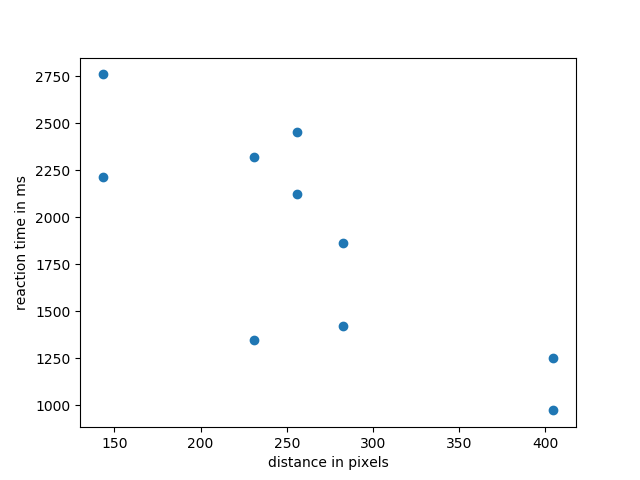
\includegraphics[width=.6\textwidth]{scatter}
	\caption{An example result of plotting the reaction time against the circle distance}
\end{figure}

\end{document}
